\subsection{API}
	La componente \textit{API} è il core dell'intera architettura; permette all'applicazione web di interfacciarsi con i due database menzionati precedentemente, oltre che con un bot Telegram.
	\newline
	La componente è stata sviluppata in Java 11, utilizzando dei framework Spring: Spring boot, Spring security, Spring kafka e Spring jpa; per l'autenticazione web è stato usato Json Web Token.

	\subsubsection{Diagramma dei package}%%%%%%%%%%%%%%OK
		\begin{figure}[H]
			\centering
			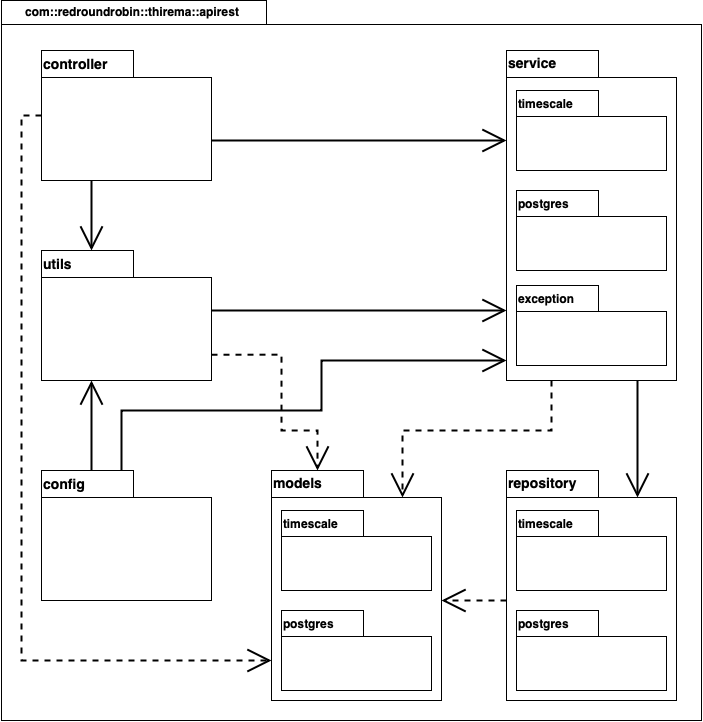
\includegraphics[scale=0.500]{res/images/API/packageAPI.png}
			\caption{Diagramma dei packages per la componente API}
			\label{Diagramma 10}
		\end{figure}

	\subsubsection{Dipendenze esterne}
		La componente \textit{API} he le seguenti dipendenze esterne:
		\begin{itemize}
			\item \textbf{Spring Boot}, che viene utilizzato per rendere le API un microservizio; 
			\item \textbf{Spring Boot Jpa}, contenuta nel framework precedente, viene utilizzata per permettere al package Repository e Config di interfacciarsi direttamente con il database;
			\item \textbf{Spring Boot Starter Security}, contenuta nel framework Spring Boot, viene utilizzata per gestire la sicurezza nell'accesso alle API;
			\item \textbf{SpringBoot Starter Test}, contenuta nel framework Spring Boot, viene utilizzata per eseguire i test.
			\item \textbf{org.Moquito}, libreria usata per fare simulare il comportamento di alcune funzioni, in fase di test.
			\item \textbf{io.jsonwebtoken}, libreria usata per la creazione di token necessari all'accesso ad aree riservate della API.
			\item \textbf{Spring Kafka}, libreria utilizzata per la comunicazione con Kafka;
			\item \textbf{Spring Doc}, libreria utilizzata per la visualizzazione delle richieste API tramite interfaccia web;
			\item \textbf{org.postgreSql.Driver}, che viene utilizzato per la connessione con DBMS di tipo Postgres; 
		\end{itemize}

	\subsubsection{Diagrammi delle classi}
		Al fine di semplificare la comprensione delle dipendenze della componente API, si è deciso di suddividere i diagrammi per package, mostrando in dettaglio quelli più significativi.

		
		\begin{figure}[H]
			\centering
			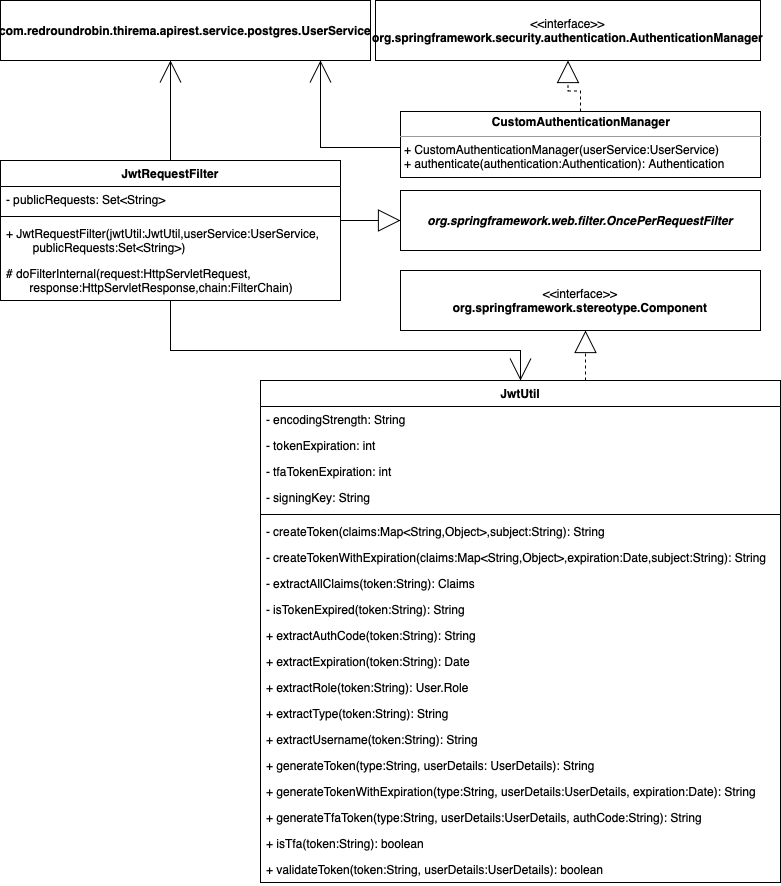
\includegraphics[scale=0.550]{res/images/API/UtilsPackage.png}
			\caption{Diagramma del package utils della componente API}
			\label{Diagramma 11}
		\end{figure}
		\begin{figure}[H]
			\centering
			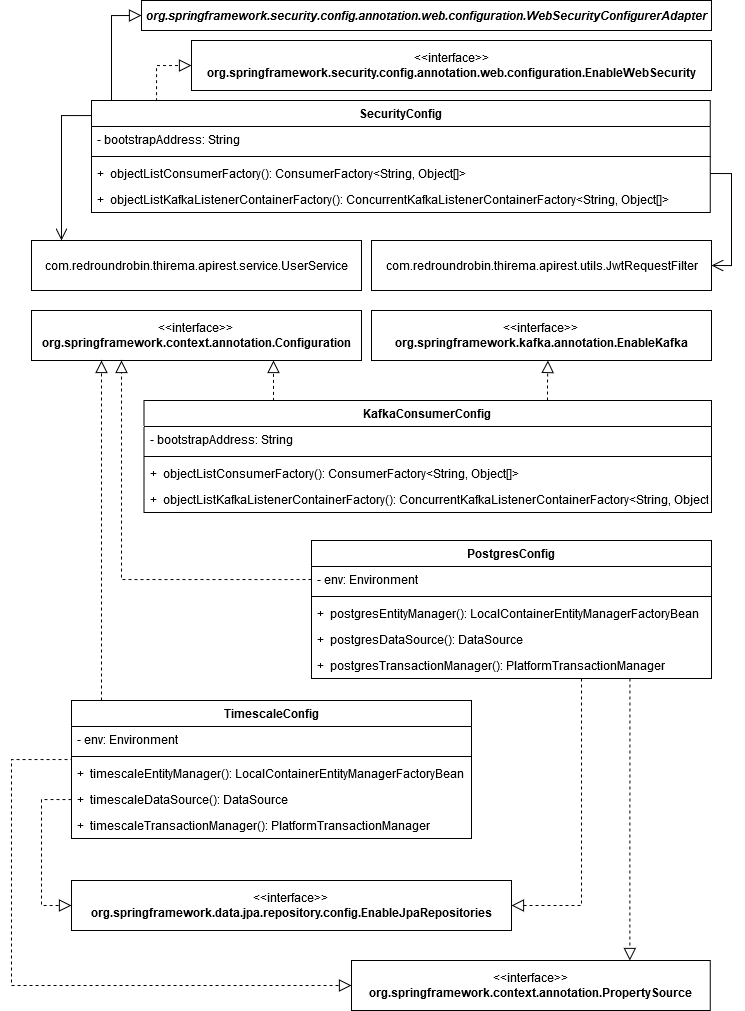
\includegraphics[scale=0.550]{res/images/API/ConfigPackage.png}
			\caption{Diagramma del package config della componente API}
			\label{Diagramma 12}
		\end{figure}
		\begin{figure}[H]
			\centering
			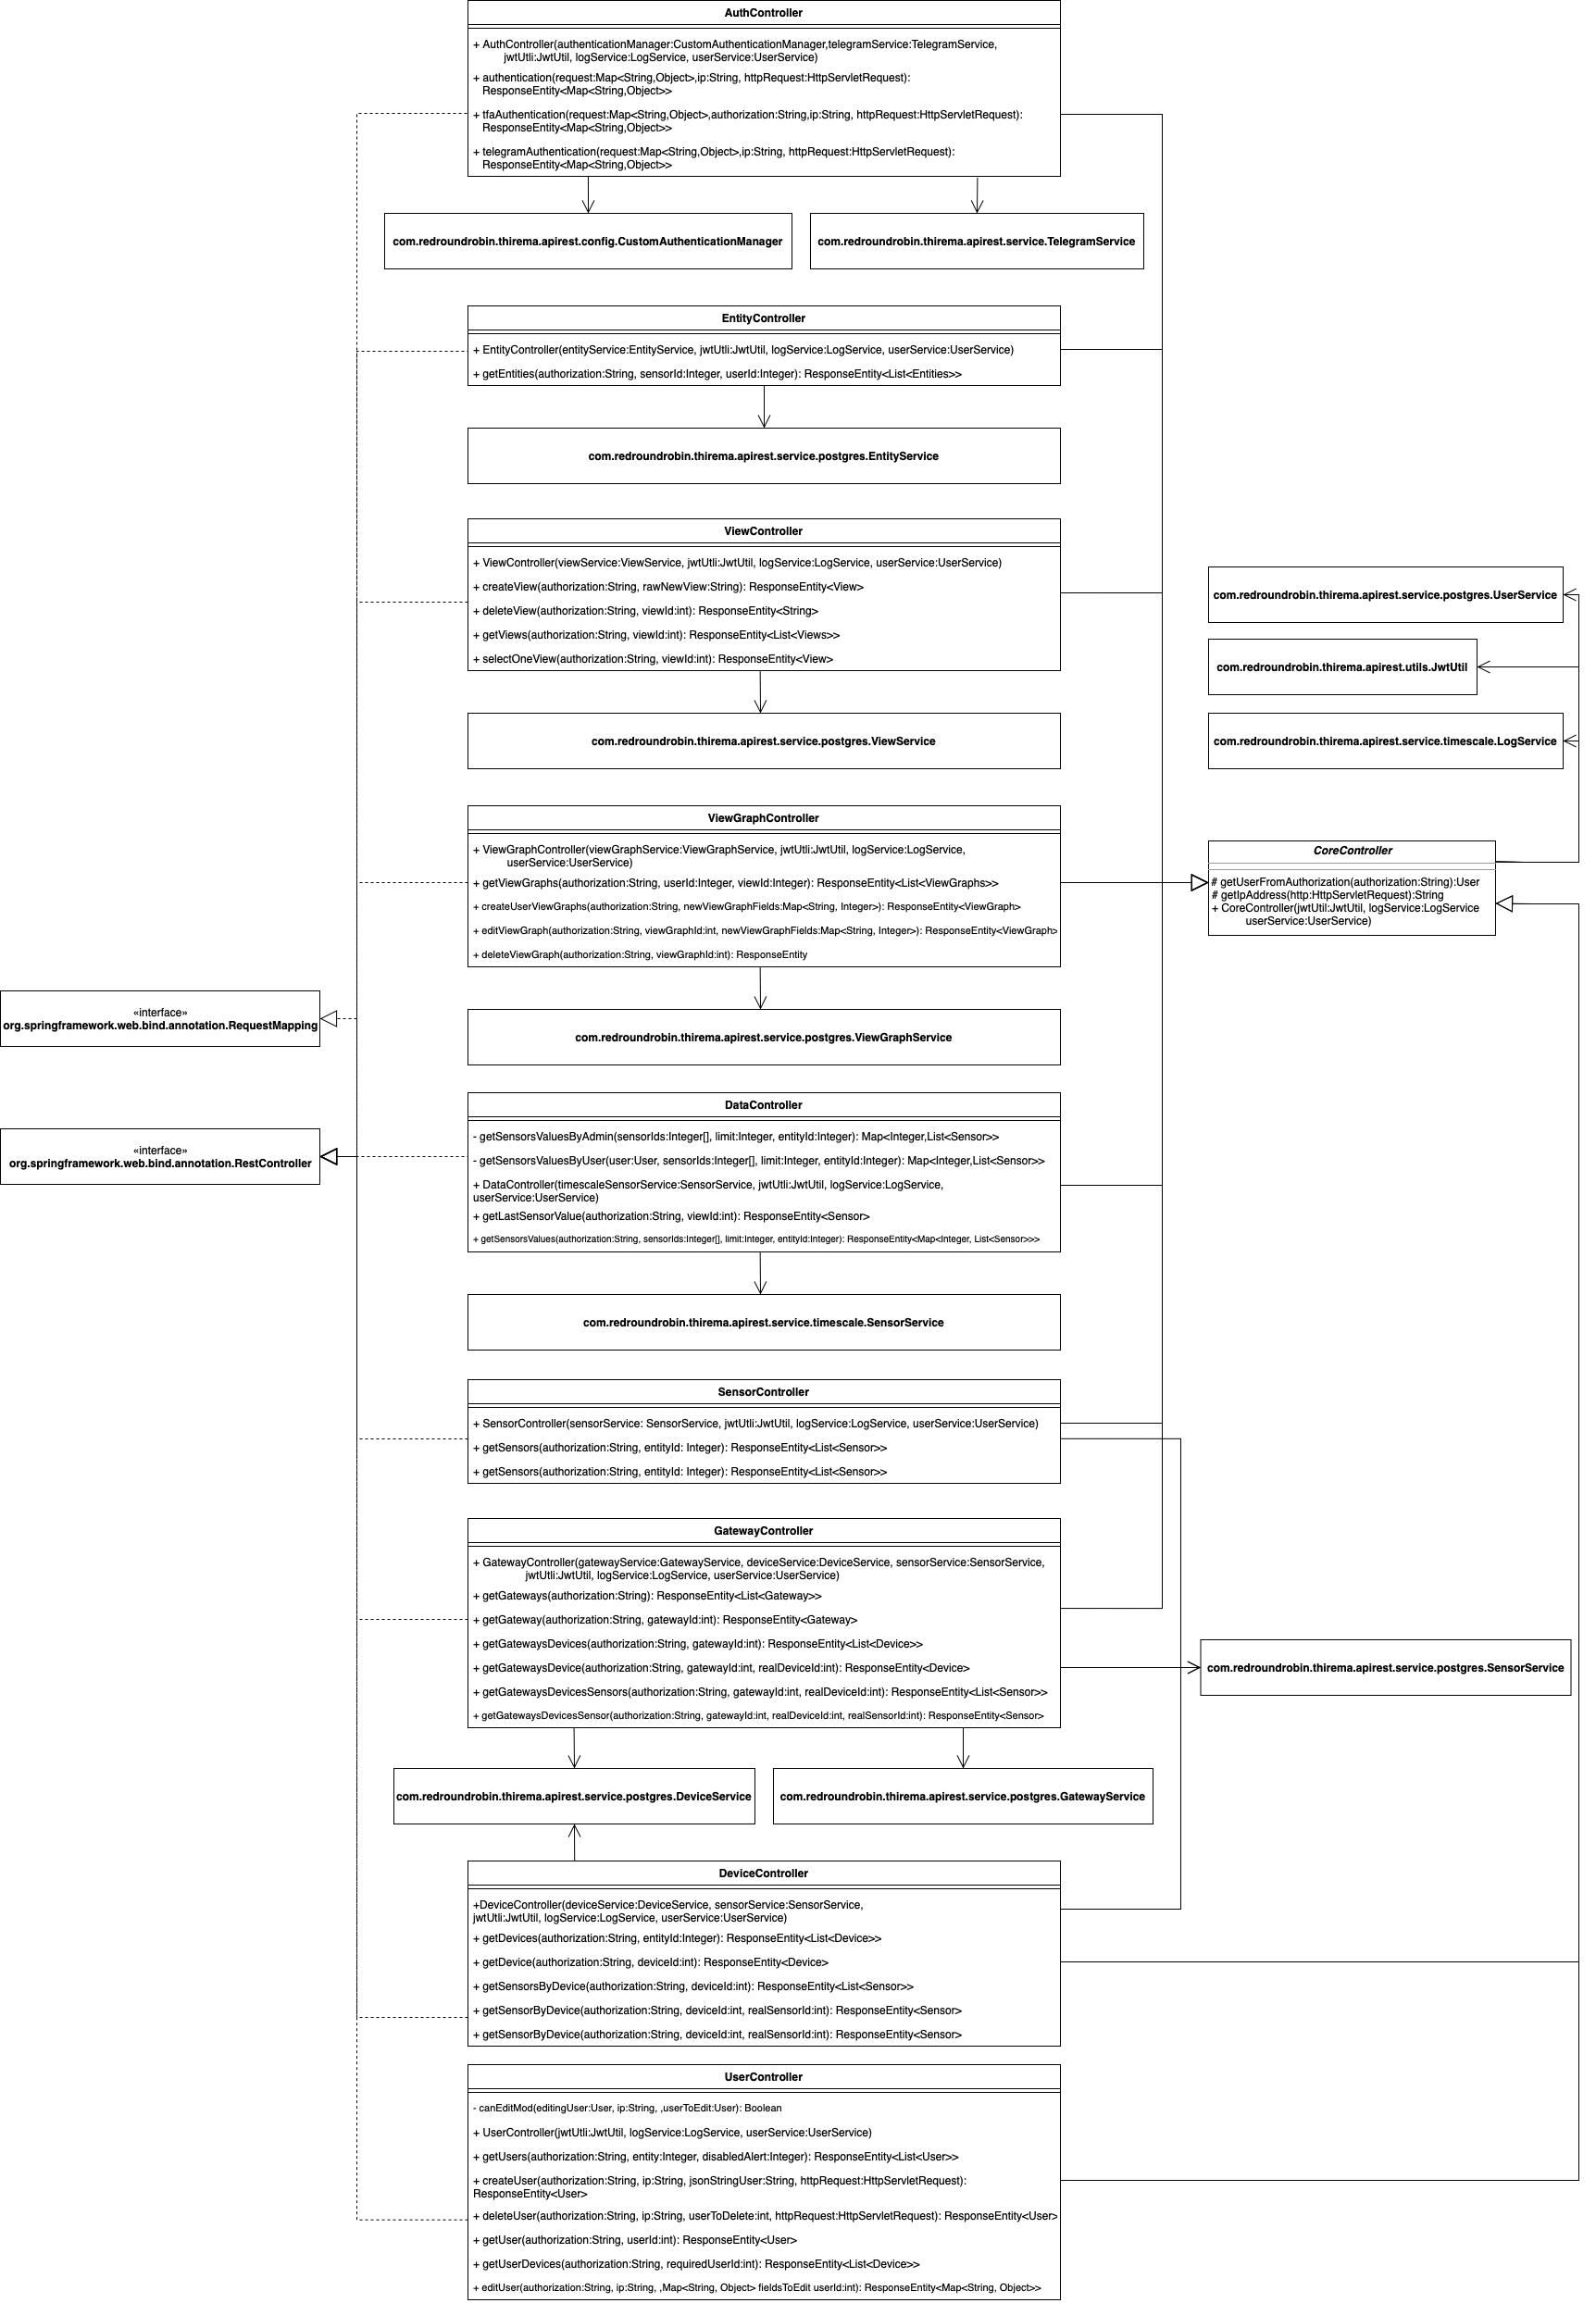
\includegraphics[scale=0.295]{res/images/API/Controllers.png}
			\caption{Diagramma del package controllers della componente API}
			\label{Diagramma 13}
		\end{figure}
		\begin{figure}[H]
			\centering
			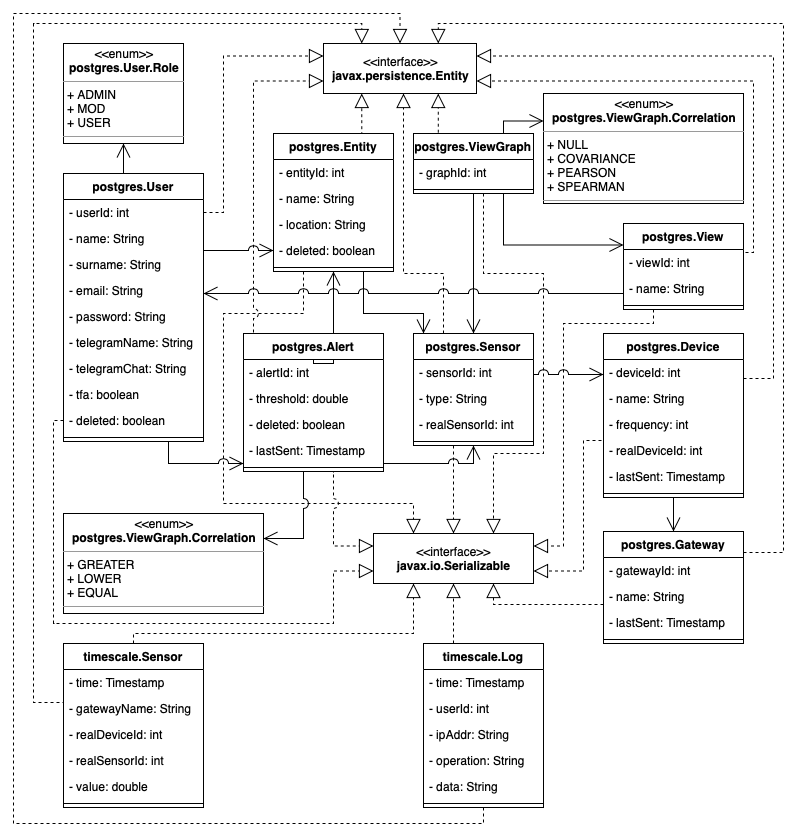
\includegraphics[scale=0.550]{res/images/API/ModelsPackage.png}
			\caption{Diagramma del package models della componente API}
			\label{Diagramma 14}
		\end{figure}
		\begin{landscape}
		\begin{figure}[H]
			\centering
			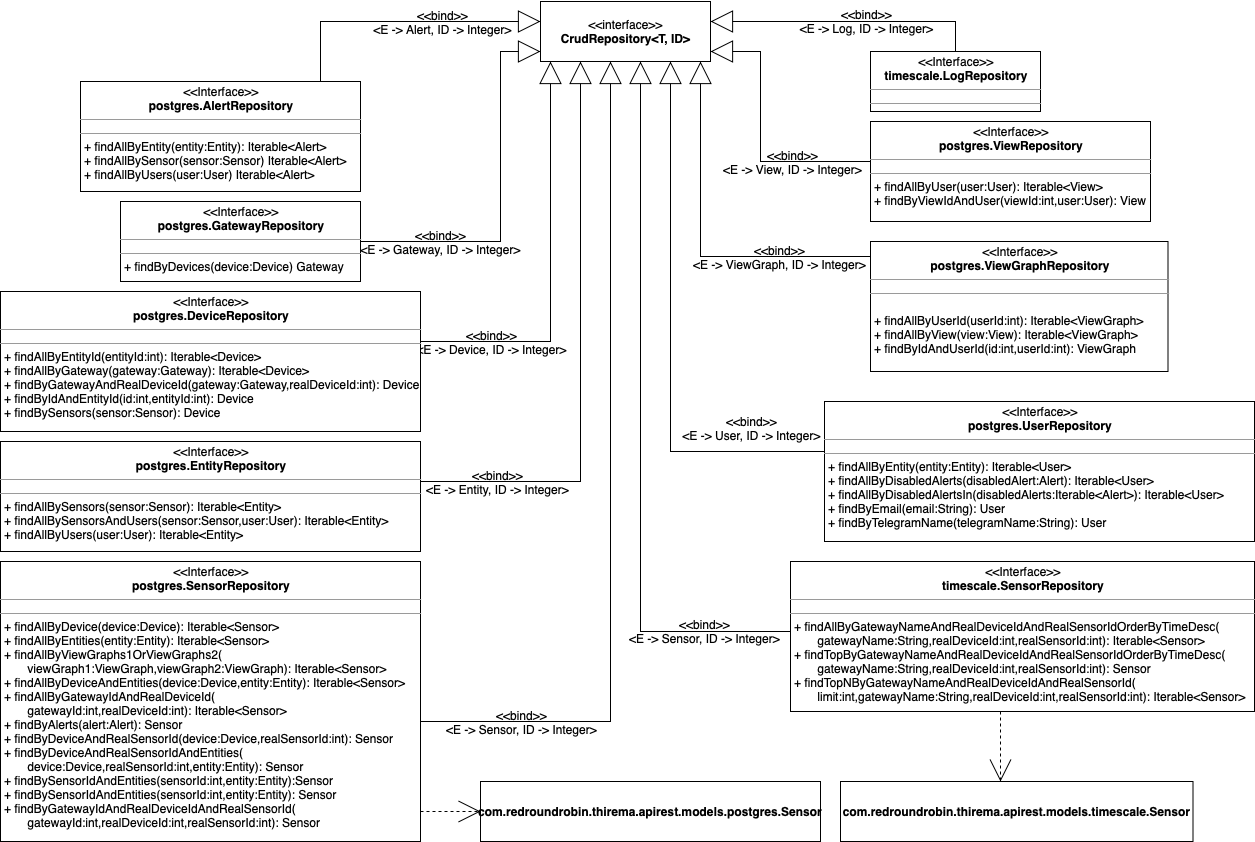
\includegraphics[scale=0.525]{res/images/API/RepositoryPackage.png}
			\caption{Diagramma del package repository della componente API}
			\label{Diagramma 15}
		\end{figure}
		\begin{figure}[H]
			\centering
			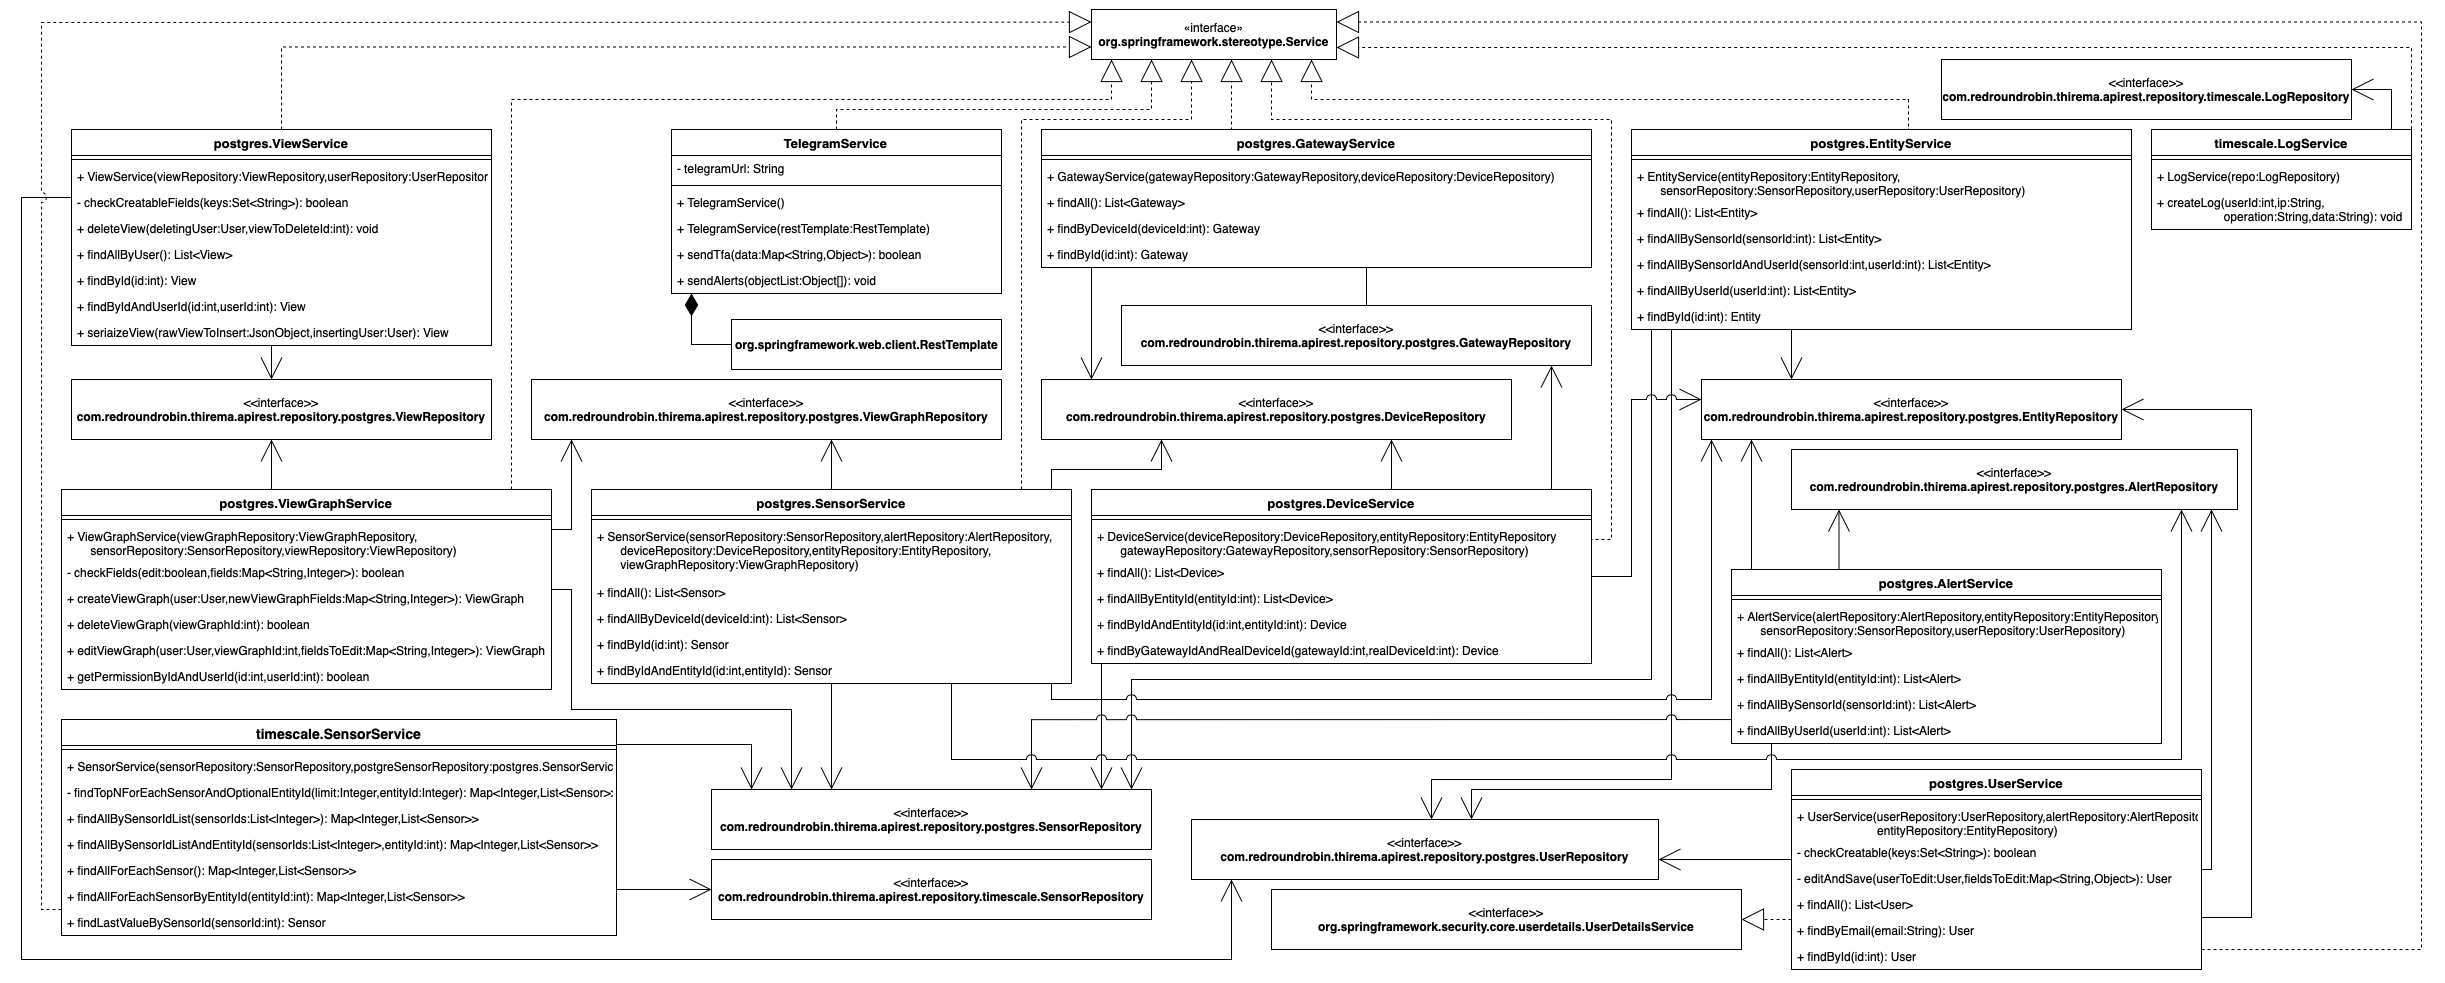
\includegraphics[scale=0.300]{res/images/API/ServicePackage.png}
			\caption{Diagramma del package service della componente API}
			\label{Diagramma 16}
		\end{figure}
		
	\subsubsection{Diagrammi di sequenza}%%%%%%%%%OK
		\begin{figure}[H]
			\centering
			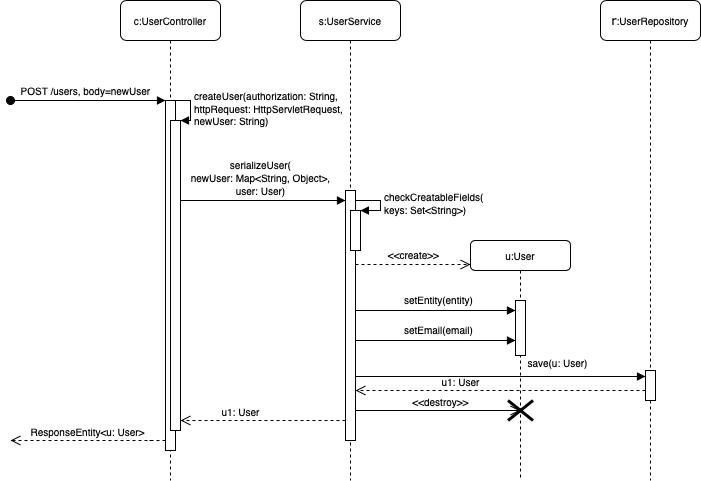
\includegraphics[scale=0.750]{res/images/API/inserimento_utente.png}
			\caption{Diagramma di sequenza che mostra l'inserimento di un utente all'interno della componente API}
			\label{Diagramma 17}
		\end{figure}
		\begin{figure}[H]
			\centering
			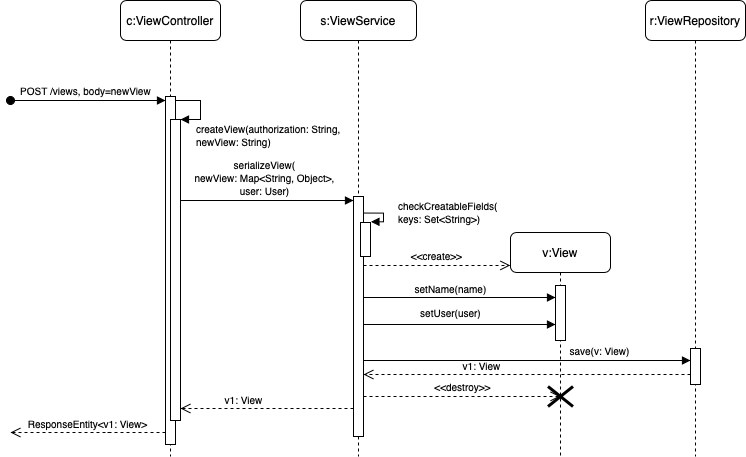
\includegraphics[scale=0.750]{res/images/API/inserimento_view.png}
			\caption{Diagramma di sequenza che mostra l'inserimento di una view all'interno della componente API}
			\label{Diagramma 18}
		\end{figure}
	\end{landscape}

	\subsubsection{Estensione}
		\paragraph{Aggiungere una richiesta API}
			Per inserire una nuova richiesta è necessario, se non si usano le classi già esistenti è necessario che la nuova classe creata che implementi l'interfaccia RestController tramite la notazione \textit{@RestController} da inserire precedentemente alla definizione della classe.
			All'interno della classe è necessario definire una funzione usando una notazione di tipo mapping, ad esempio "@GetMapping", inserendo all'interno delle parentesi tonde la stringa associata all'URI della richiesta che si vuole implementare.
			Ad esempio:
			\begin{verbatim}
			@GetMapping(value = \{"/{deviceId:.+}/sensors"\})
			\end{verbatim}
			Per esporre una risorsa senza necessità di autenticazione è necessario aggiungere all'array publicRequests l'URL della richiesta. L'array publicRequests è un attributo della classe SecurityConfig.